\documentclass[12pt, a4paper, twoside, article]{memoir}
\usepackage[a4paper, total={6.5in, 8in}]{geometry}
\usepackage[table,xcdraw]{xcolor}
\usepackage[utf8]{inputenc}
\usepackage[english]{babel}
\usepackage[T1]{fontenc}
\usepackage[final]{microtype}
\usepackage{amsmath,amssymb}
\usepackage{bm}
\usepackage{amsthm}
\usepackage{mathtools}
\usepackage{listings}
\usepackage{graphicx}
\usepackage{amsmath}
\usepackage{float}
\makeatletter
\renewcommand*\env@matrix[1][*\c@MaxMatrixCols c]{%
	\hskip -\arraycolsep
	\let\@ifnextchar\new@ifnextchar
	\array{#1}}
\makeatother
\usepackage[colorlinks=true,linkcolor=blue,urlcolor=black]{hyperref}
\usepackage{bookmark}
\DeclareMathSymbol{*}{\mathbin}{symbols}{"01}
\usepackage{color}

\usepackage[sc]{mathpazo}
\renewcommand{\ttdefault}{txtt}
\linespread{1.15}
\renewcommand{\chapnamefont}{\large\em}
\newcommand{\regi}[1]{ %
	{%
		\centering
		\em #1
		\par
	}
}

\setcounter{tocdepth}{3}
\setcounter{secnumdepth}{3}

% Fancy chapters
\usepackage{tikz}
\makechapterstyle{box}{
	\renewcommand*{\printchaptername}{}
	\renewcommand*{\chapnumfont}{\HUGE\bfseries}
	\renewcommand*{\printchapternum}{
		\flushright
		\begin{tikzpicture}
			\draw[fill,color=black] (0,0) rectangle (2cm,2cm);
			\draw[color=white] (1cm,1cm) node { \chapnumfont\thechapter };
		\end{tikzpicture}
	}
	\renewcommand*{\chaptitlefont}{\HUGE\bfseries}
	\renewcommand*{\printchaptertitle}[1]{\flushright\chaptitlefont##1}
}
\chapterstyle{box}



% Fancy headers
\usepackage{fancyhdr}

\pagestyle{fancy}
\fancyhf{}
\fancyhead[LE,RO]{}
\fancyhead[RE,LO]{\textsc{Marc Breiner Sørensen}}
\fancyfoot[RE,LO]{\thepage}
\fancyfoot[LE,RO]{ \small\leftmark}

\renewcommand{\headrulewidth}{2pt}
\renewcommand{\footrulewidth}{1pt}


% Fancy breadtext
%\usepackage{ebgaramond, fontspec}
%\setmainfont{EB Garamond}
%\renewcommand{\familydefault}{\ebgaramond}
%\usepackage {xcolor}

\title{\color{white}\textsc{Characterization and testing of CCDs for use in astronomical satellite missions
		 \\ \normalsize Requirements input for the STEP mission}}	
\author{\color{white}\normalsize \textbf{\textsc{Marc Breiner Sørensen}}\\\color{white}\normalsize 201708238\\ \color{white}\normalsize \textbf{1. June 2022}\\\\
	\color{white}\normalsize Supervisors: \textbf{Hans Kjeldsen} \& \textbf{Mads Fredslund Andersen}\\
	\color{white}\normalsize Department of Physics and Astronomy, Aarhus University }
\date{\color{white}\textsc{\textsf{%\today
}}}
\usepackage{minted}
\usepackage{tcolorbox}
\tcbuselibrary{minted,breakable,xparse,skins}

\definecolor{bg}{gray}{0.95}
\DeclareTCBListing{mintedbox}{O{}m!O{}}{%
	breakable=true,
	listing engine=minted,
	listing only,
	minted language=#2,
	minted style=default,
	minted options={%
		linenos,
		gobble=0,
		breaklines=true,
		breakafter=,,
		fontsize=\small,
		numbersep=8pt,
		#1},
	boxsep=0pt,
	left skip=0pt,
	right skip=0pt,
	left=25pt,
	right=0pt,
	top=3pt,
	bottom=3pt,
	arc=5pt,
	leftrule=0pt,
	rightrule=0pt,
	bottomrule=2pt,
	toprule=2pt,
	colback=bg,
	colframe=black!70,
	enhanced,
	overlay={%
		\begin{tcbclipinterior}
			\fill[darkgray!20!white] (frame.south west) rectangle ([xshift=20pt]frame.north west);
	\end{tcbclipinterior}},
	#3}
\usepackage{mwe}
\newenvironment{changemargin}[2]{%
	\begin{list}{}{%
			\setlength{\topsep}{0pt}%
			\setlength{\leftmargin}{#1}%
			\setlength{\rightmargin}{#2}%
			\setlength{\listparindent}{\parindent}%
			\setlength{\itemindent}{\parindent}%
			\setlength{\parsep}{\parskip}%
		}%
		\item[]}{\end{list}}
\usepackage{eso-pic,graphicx}
% Multi-file preamble stuff
\graphicspath{{images/}}
\usepackage{subfiles} % Best loaded last in the preamble
\begin{document}
	\begin{changemargin}{-0.225cm}{-1cm}
	\AddToShipoutPictureBG*{\centering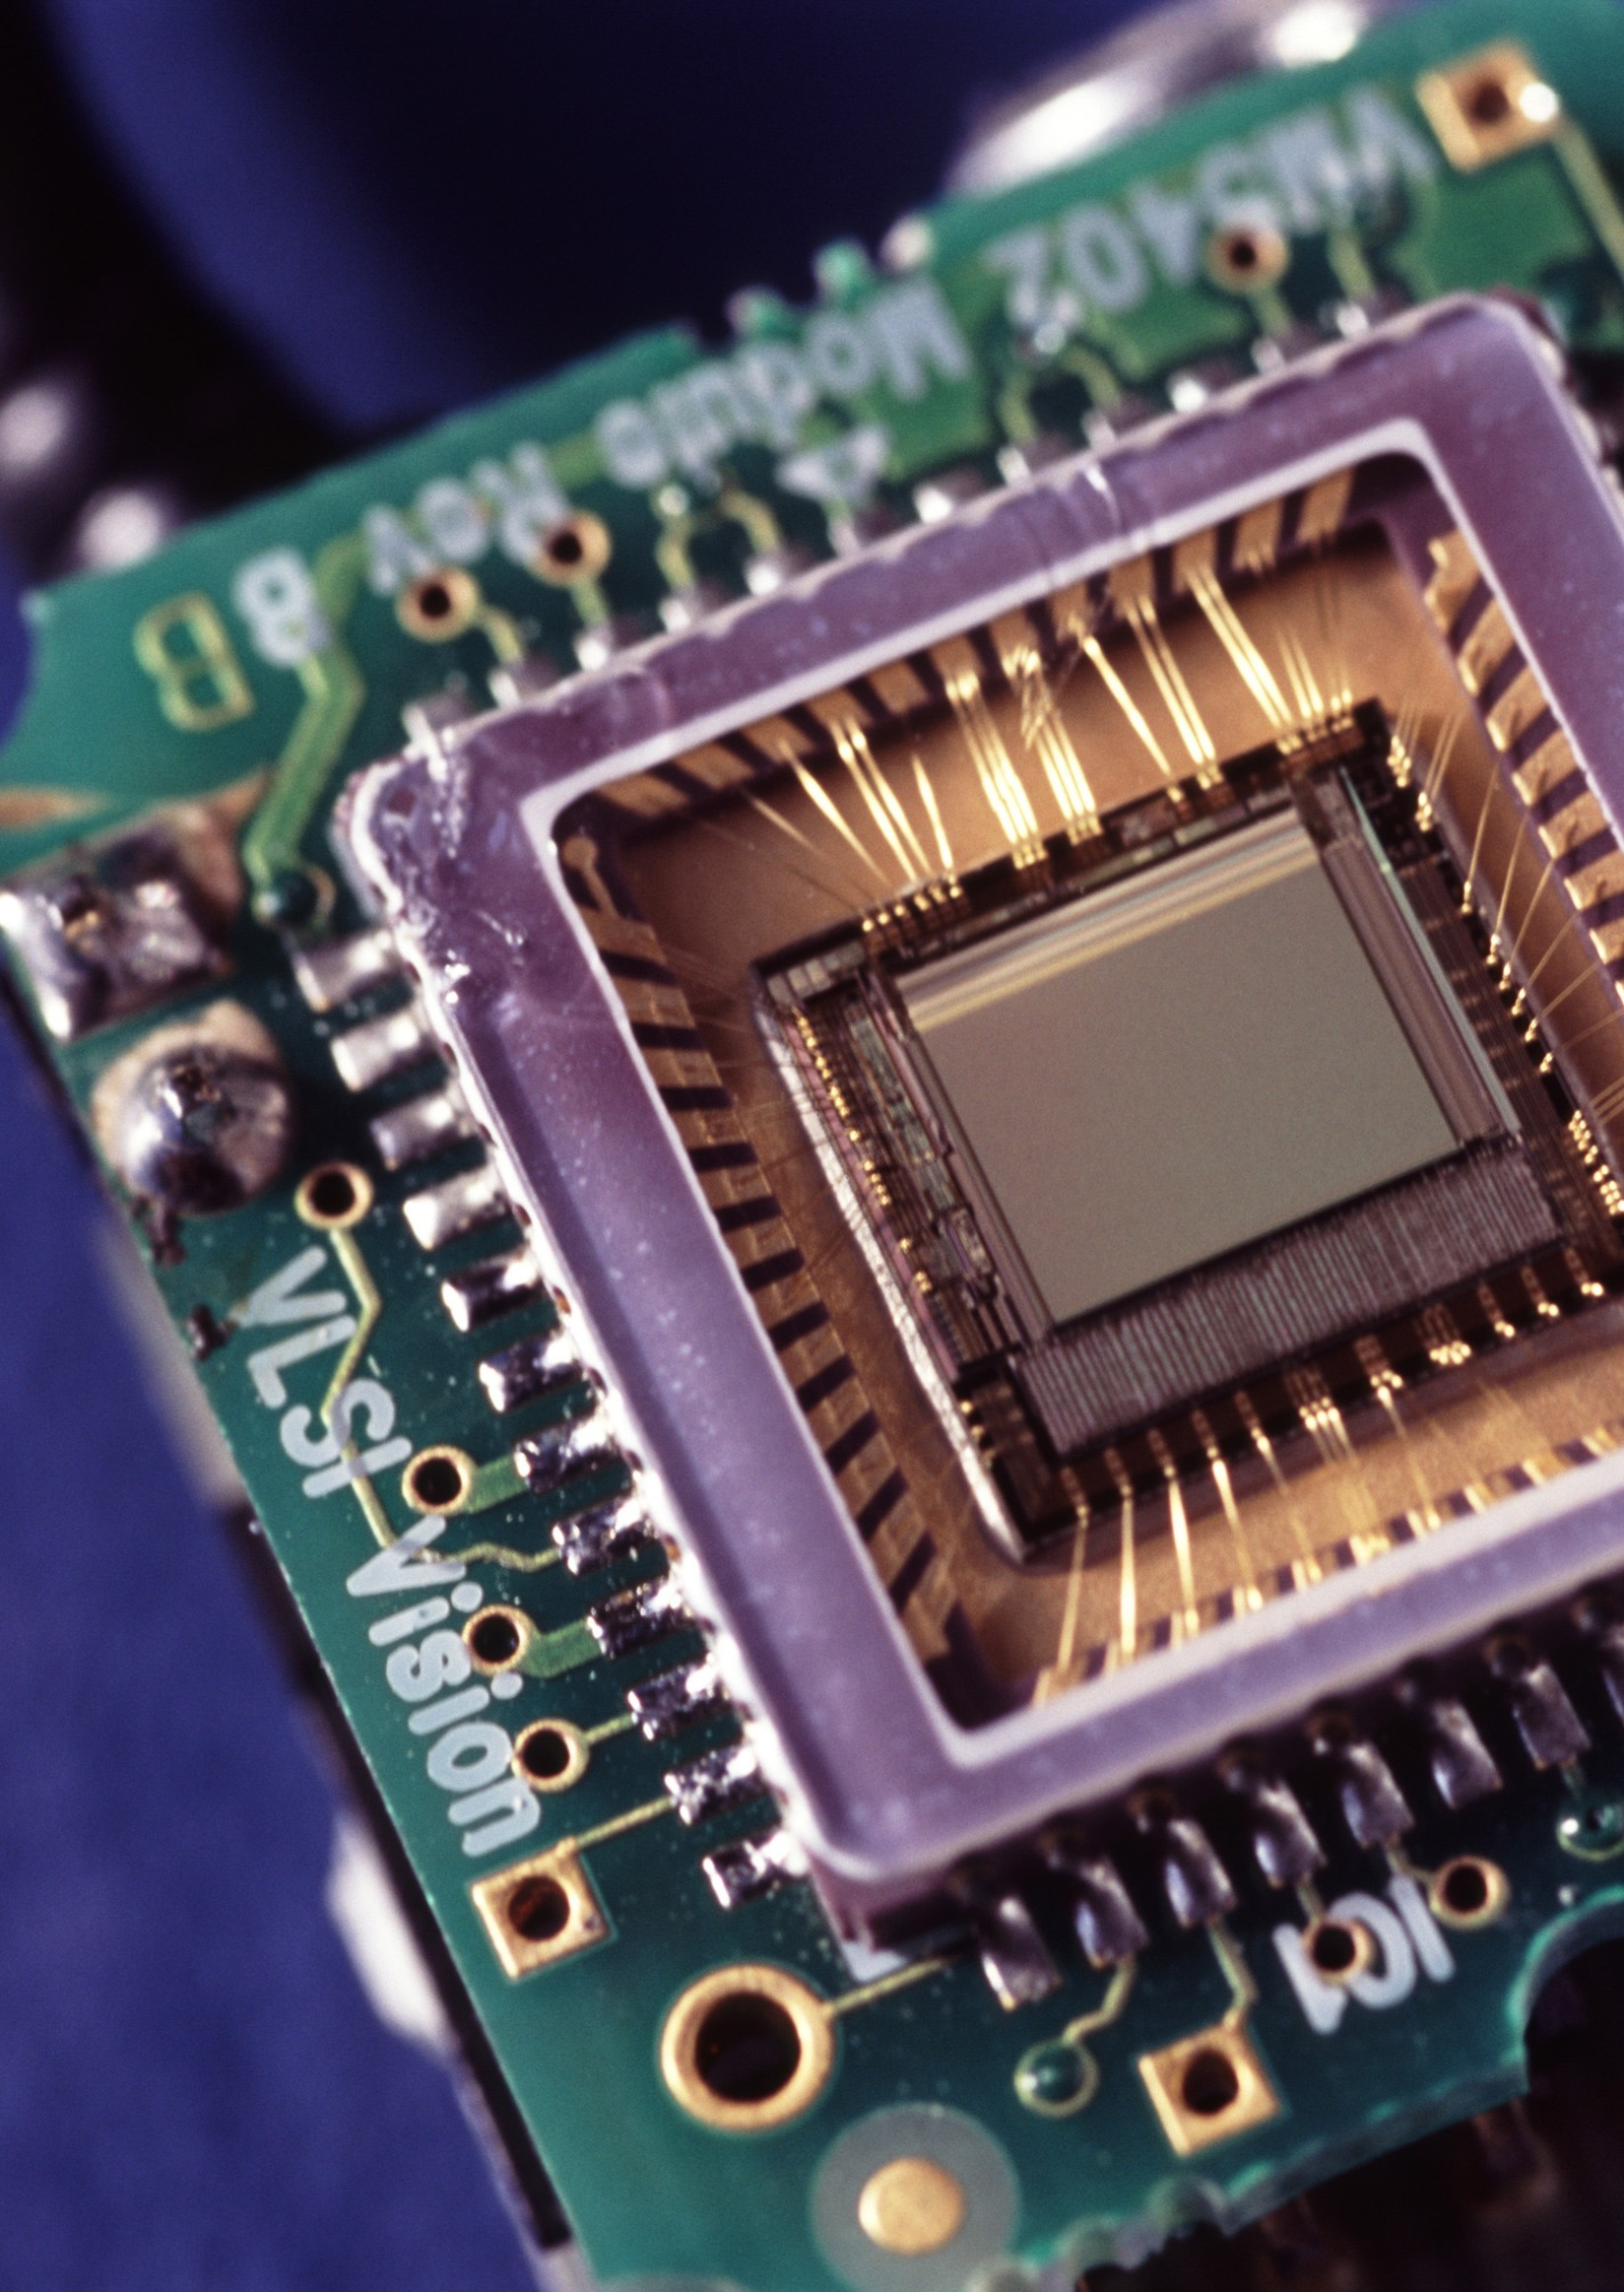
\includegraphics[width=\paperwidth,height=\paperheight]{ccd_sensor_bg.jpg}};
	{\centering
	\begin{tcolorbox}[colback = black, colframe = black, sharpish corners]
	\maketitle
	\pagenumbering{gobble}
\end{tcolorbox}}
\end{changemargin}	
	%\begin{figure}[h!]
	%	\centering
		%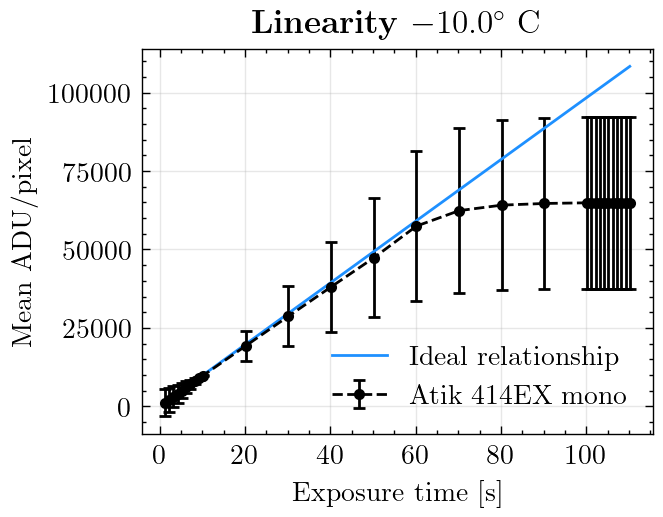
\includegraphics[width=0.58\textwidth]{/home/marc/Dropbox/STEP_Speciale_Marc/linearity.png}
%		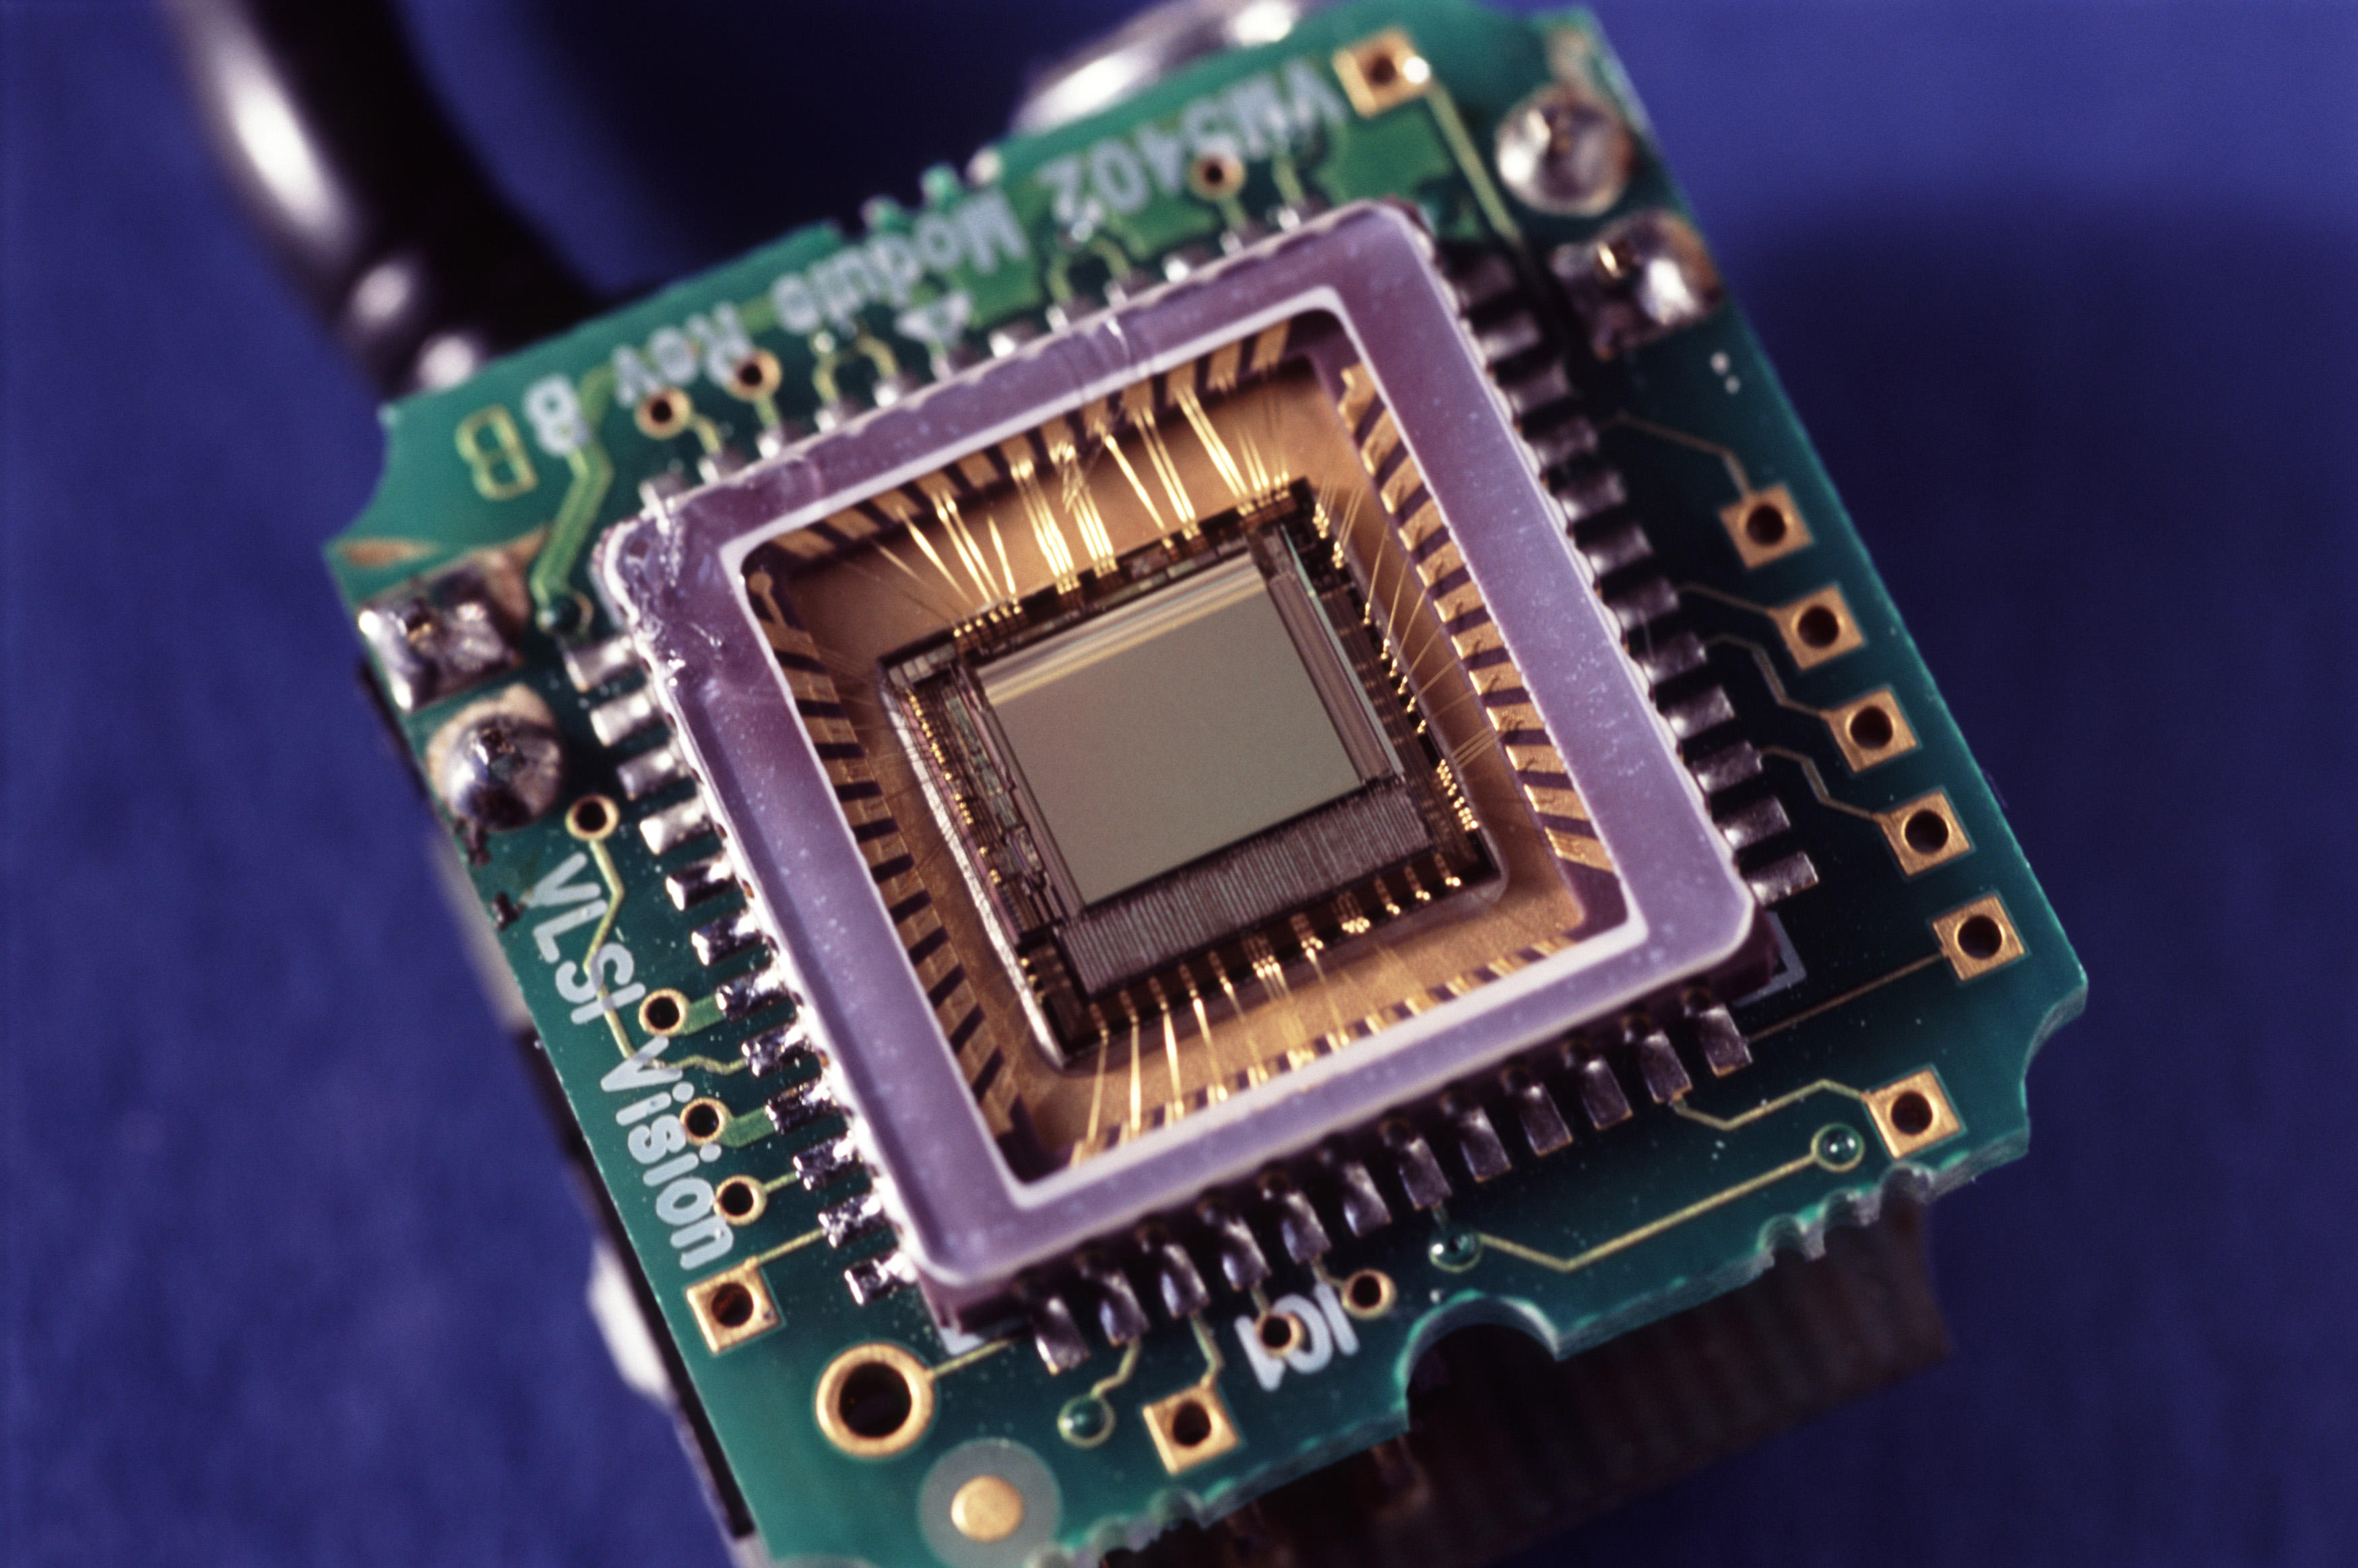
\includegraphics[width=0.8\textwidth]{ccd_sensor.jpg}
%	\end{figure}
	\thispagestyle{empty}
	
	\clearpage 
	\thispagestyle{empty}
	\vspace*{5cm}
	\noindent \textbf{Dansk titel}: \\ \textit{Karakteristik og test af CCD'er til brug i astronomiske satellitmissioner: Input til STEPs kravsspecifikationer}\\
	\noindent  \color{white}.\\ \color{black}
	\noindent\copyright 2022 Marc Breiner Sørensen\\
	\noindent Department of Physics and Astronomy\\
	\noindent Aarhus University\\
	\noindent Ny Munkegade 120\\
	\noindent DK-8000 Aarhus C\\
	\noindent Denmark\\
	\noindent  \color{white}.\\ \color{black}
	\noindent \textbf{Email:} \texttt{\url{mbsoerensen@post.au.dk}} or \texttt{\url{achnms3@gmail.com}}\\
	\noindent \textbf{LinkedIn:} \texttt{\url{https://www.linkedin.com/in/marc-breiner-s\%C3\%B8rensen-47772768/}}\\\\
	\noindent 2nd. ed. \today
	
	\clearpage
	\pagenumbering{roman}
	\tableofcontents
	\thispagestyle{empty}
	
	\clearpage
	
	
	\subfile{sections/abstract}
	\clearpage
	
	\pagenumbering{arabic}
	\subfile{sections/introduction}
	\clearpage
	\thispagestyle{empty}
	\mbox{}
	\clearpage
	
	
	\subfile{sections/theory}\clearpage
	%\thispagestyle{empty}
	%\mbox{}
	%\clearpage
	
	\subfile{sections/methods}\clearpage
	\thispagestyle{empty}
	\mbox{}
	\clearpage
	
	\subfile{sections/missionreq}
	\clearpage
	\thispagestyle{empty}
	\mbox{}
	\clearpage
	
	\subfile{sections/discuscons}
	\clearpage
	
	
	\clearpage
	\bibliographystyle{plain} % We choose the &quot;plain&quot; reference style
	\bibliography{refs} % Entries are in the &quot;refs.bib&quot; file</code></pre>
	
	\clearpage
	\subfile{sections/appendix}
	
	\clearpage
	\thispagestyle{empty}
	\AddToShipoutPictureBG*{\centering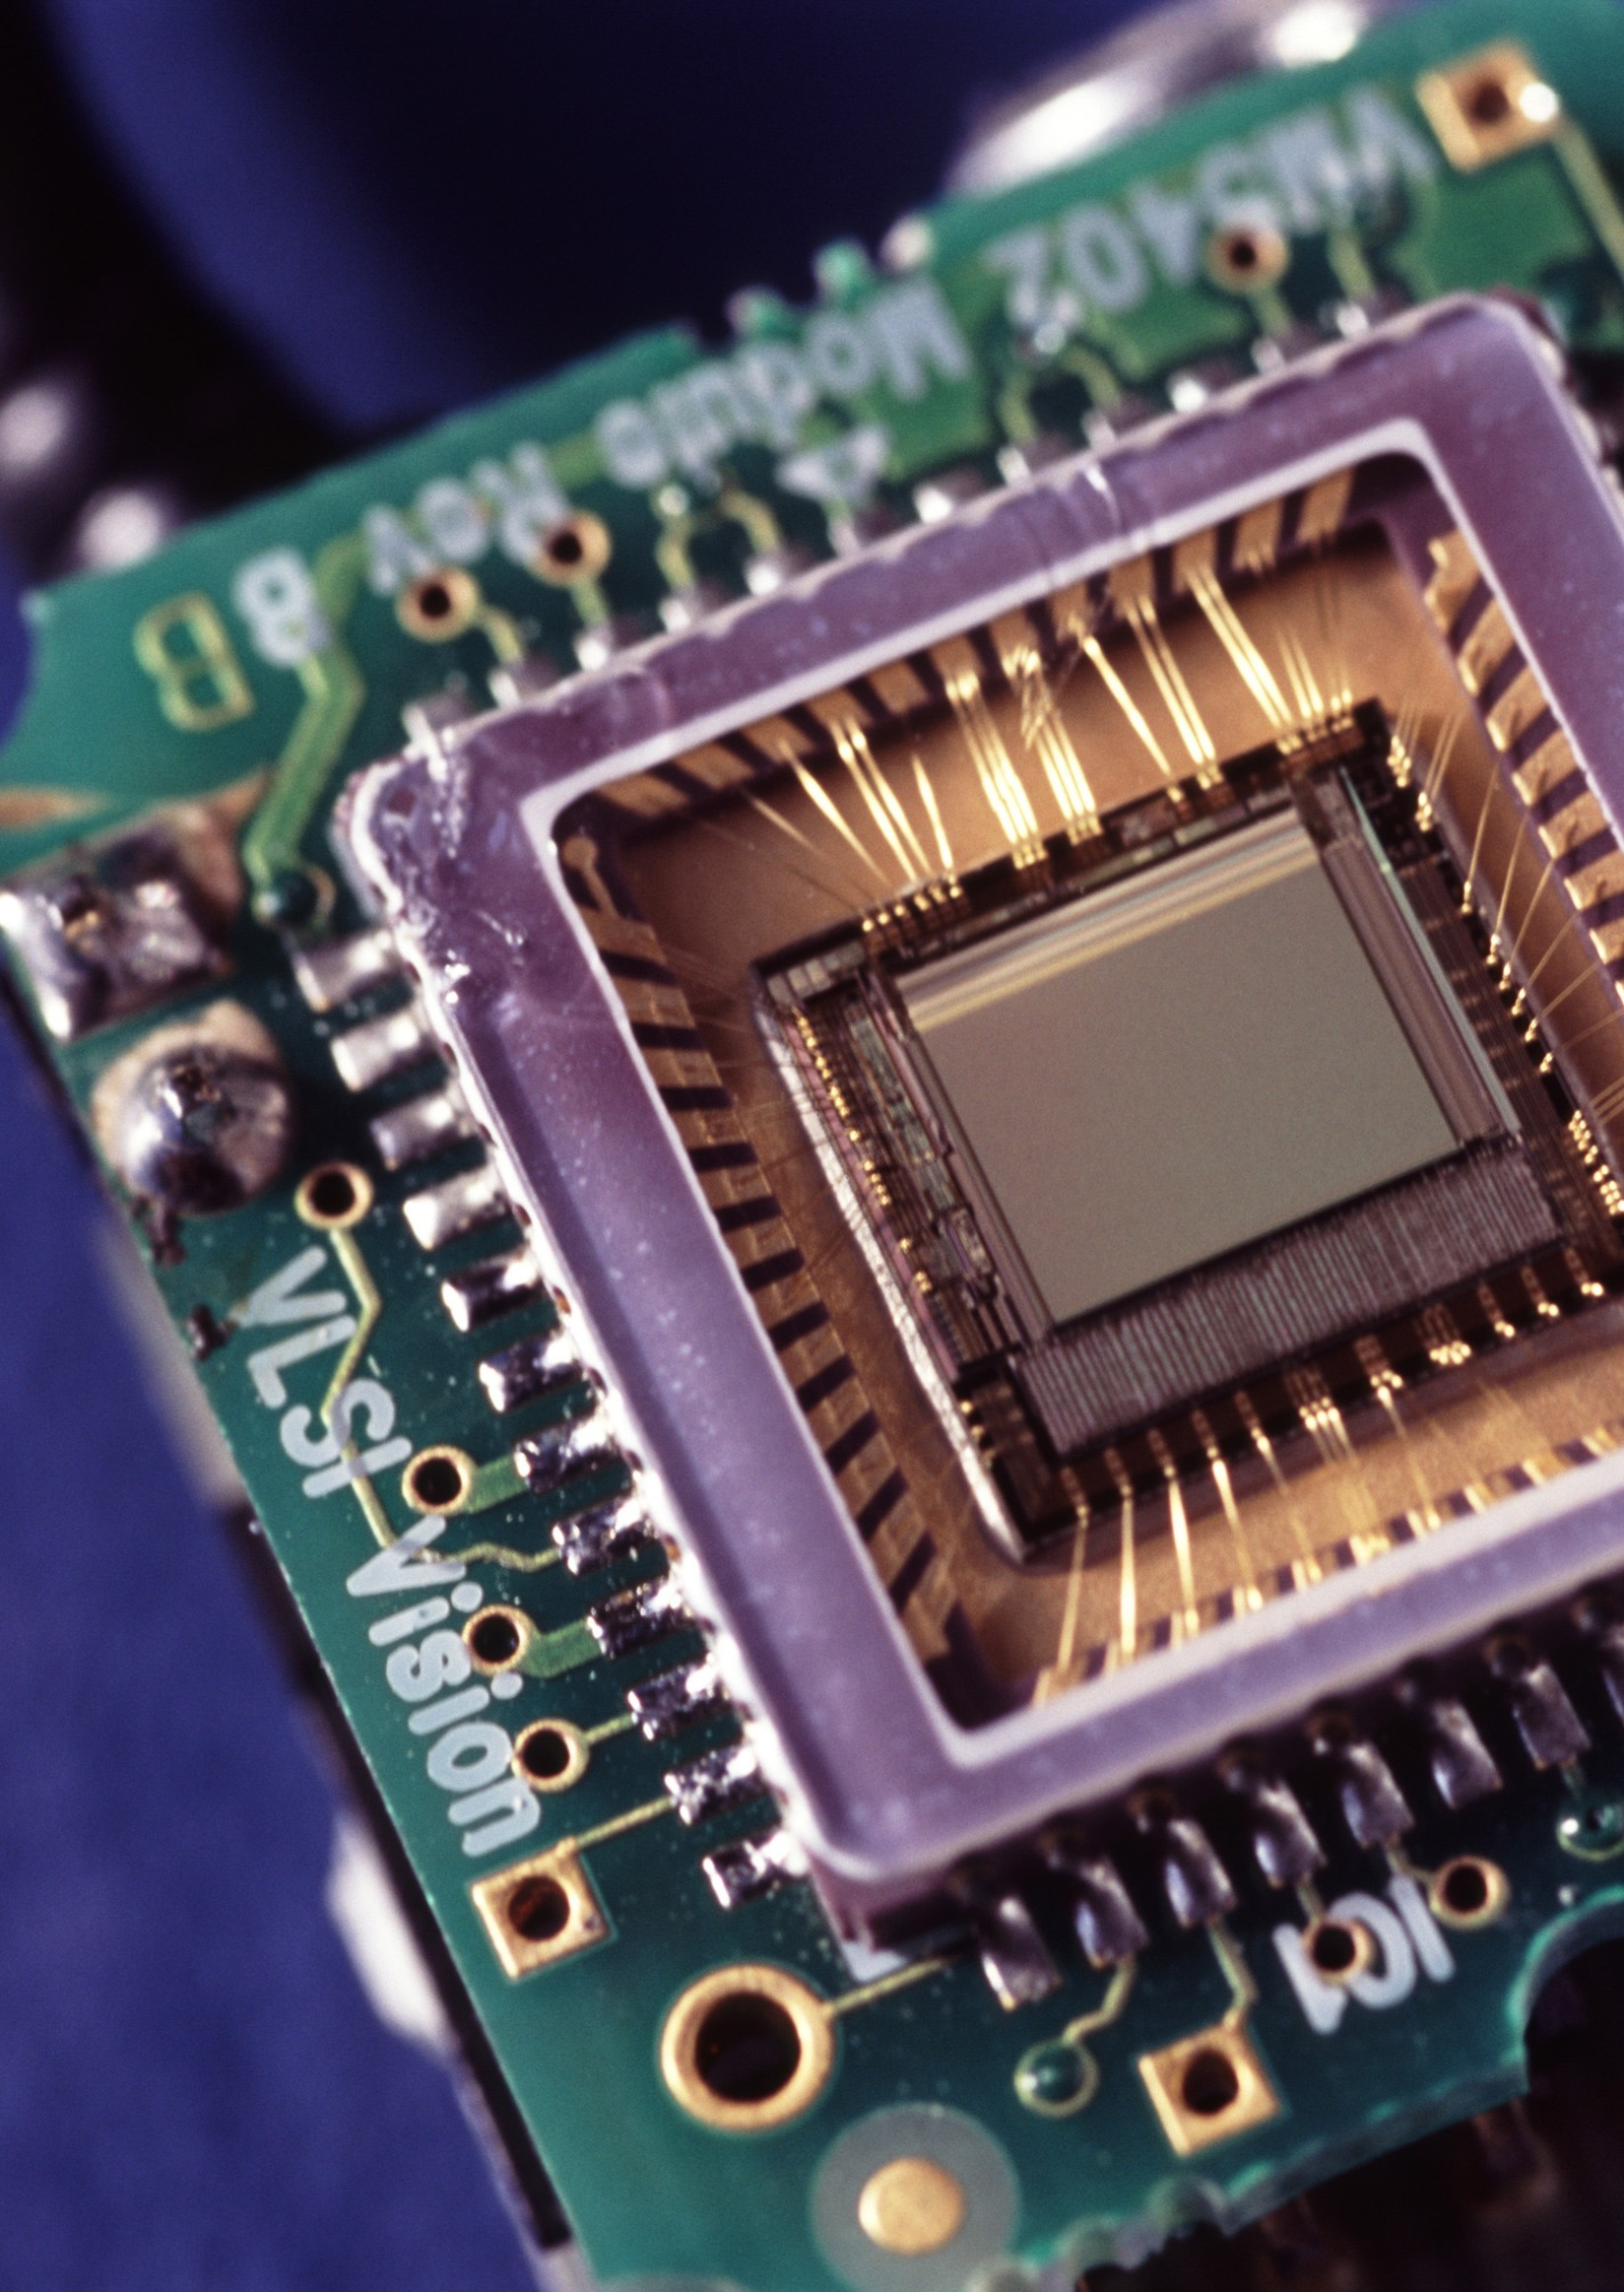
\includegraphics[width=\paperwidth,height=\paperheight]{ccd_sensor_bg.jpg}};
	
	\begin{changemargin}{-0.225cm}{-1cm}
	\begin{tcolorbox}[colback = black, colframe = black, sharpish corners]
		\color{white} This work is a study of the usage of CCDs in astronomical satellite missions. The main focus is on the proposed Danish astronomical microsatellite mission, STEP. STEP will provide photometric time-series data of stars to study exoplanet transits and stellar properties. Scientific requirements for the mission were derived from a case study of systemic effects in the Kepler seasonal data given in \cite{hatp7}. The two requirements are a photometric precision of at least  $5*10^{-4}$ in the linearity curve of the CCD and a maximum flux variability resulting from spacecraft attitude errors of $10^{-4}$. A characterization procedure was designed and validated. Here it is found that, for the detector used to develop the test procedure, to meet this requirement, it is adequate to use $10$ repeats of the measurement of the linearity curve. Arbitrary precision can be obtained for a given detector with enough measurements. A test to output technical requirements for the ADCS subsystem was developed and verified. For requirements to be met the light was allowed to move at most $ 0.2 $ pixels during observation. If optics like those used on the TESS space mission are assumed, this requirement corresponds to stabilizing the satellite attitude to within $4.2''$ during observation. 
		
		In the presently developed characterization procedure, a simple setup of inexpensive equipment found in any university teaching lab, is used. The light source used is ambient room lighting from a fluorescent bulb. A measurement acquisition scheme to prevent effects from drifting of the intensity, is presented along with a detector time calibration. The consequence is that this characterization may be performed using an arbitrary light source. The light soure does not need to be calibrated, enabling small missions with constrained budgets to characterize and test their detectors thoroughly. In addition, the characterization may be redone or validated in space, and the author suggests an approach using the moon as a light source.
		\pagenumbering{gobble}
	\end{tcolorbox}
	
\end{changemargin}	
\end{document}